%%%%%%%%%%%%%%%%%%%%%%%%%%%%%%%%%%%%%%%%%
% Document Author: Plinio H. Vargas
% Course: CS-532, Spring 2016 at Old Dominion University
%
% Structured General Purpose Assignment
% LaTeX Template
%
% This template has been downloaded from:
% http://www.latextemplates.com
%
% Original template author:
% Ted Pavlic (http://www.tedpavlic.com)
%
% Note:
% The \lipsum[#] commands throughout this template generate dummy text
% to fill the template out. These commands should all be removed when 
% writing assignment content.
%
%%%%%%%%%%%%%%%%%%%%%%%%%%%%%%%%%%%%%%%%%
%----------------------------------------------------------------------------------------
%	PACKAGES AND OTHER DOCUMENT CONFIGURATIONS
%----------------------------------------------------------------------------------------

\documentclass{article}

\usepackage{fancyhdr} % Required for custom headers
\usepackage{lastpage} % Required to determine the last page for the footer
\usepackage{extramarks} % Required for headers and footers
\usepackage{listings}
\usepackage{graphicx} % Required to insert images
\usepackage{lipsum} % Used for inserting dummy 'Lorem ipsum' text into the template
\usepackage[bookmarks,bookmarksopen,bookmarksdepth=2]{hyperref} % for bookmarks
\usepackage{enumerate}
\usepackage{csquotes} % for quoting things
\usepackage{multirow}
\usepackage{amsmath}
\usepackage{caption}
\usepackage{navigator}%\usepackage{caption}
\usepackage[shortlabels]{enumitem}
\usepackage{enumitem}
\usepackage{lmodern}
\usepackage[utf8]{inputenc}
%\usepackage[table]{xcolor}% http://ctan.org/pkg/xcolo
\usepackage[dvipsnames]{xcolor}
\usepackage{longtable}
\usepackage{textcomp}
\usepackage{url}
\usepackage{import}
\usepackage{float}
\usepackage{dashrule} % for dashline
\usepackage{keystroke}
\usepackage{amssymb}

\lstdefinestyle{numbers}
{ frame=tb,
  language=python,
  aboveskip=3mm,
  belowskip=3mm,
  showstringspaces=false,
  columns=flexible,
  basicstyle={\small\ttfamily},
  numbers=left,
  numberstyle=\tiny\color{gray},
  keywordstyle=\color{blue},
  commentstyle=\color{OliveGreen},
  stringstyle=\color{purple},
  breaklines=true,
  breakatwhitespace=true,
  tabsize=3
}

\lstdefinestyle{nonumbers}
{ frame=shadowbox,
  language=python,
  aboveskip=3mm,
  belowskip=3mm,
  showstringspaces=false,
  columns=flexible,
  basicstyle={\small\ttfamily},
  numbers=none,
  numberstyle=\tiny\color{gray},
  keywordstyle=\color{blue},
  commentstyle=\color{OliveGreen},
  stringstyle=\color{purple},
  breaklines=true,
  breakatwhitespace=true,
  tabsize=3
}

\lstdefinestyle{mybox}
{
	basicstyle={\small\ttfamily},
    numbers=left,
    numberstyle=\tiny\color{gray},
    stepnumber=1,
    numbersep=5pt,
    showspaces=false, % don't show spaces by adding underscores
    showstringspaces=false, % don't underline spaces in strings
    showtabs=false, % don't show tabs with underscores
    frame=shadowbox,
    tabsize=4,
    captionpos=b,
    breaklines=true,
    breakatwhitespace=false,
  	keywordstyle=\color{blue},
	commentstyle=\color{OliveGreen},
  	stringstyle=\color{purple},    
    rulesepcolor=\color{red!20!green!20!blue!20},
    numberbychapter=false,
    stringstyle=\color{purple},
}


\providecommand{\providehyphenmins}[2]{}

% Margins
\topmargin=-0.45in
\evensidemargin=0in
\oddsidemargin=0in
\textwidth=6.5in
\textheight=9.0in
\headsep=0.25in 

\linespread{1.1} % Line spacing
\newcommand*{\medtau}{\mathbin{\scalebox{1.5}{$\tau$}}}% increase size of tau
\newcommand*{\medtaub}{\mathbin{\scalebox{1.5}{$\tau_b$}}}% increase size of tau_b
\newcommand\multibrace[3]{\rdelim\}{#1}{3mm}[\pbox{#2}{#3}]}

% Set up the header and footer
\pagestyle{fancy}
\lhead{\hmwkAuthorName} % Top left header
\chead{\hmwkShortClass\ (\hmwkClassInstructor\ \hmwkClassTime): \hmwkShortTitle} % Top center header
%\rhead{\firstxmark} % Top right header
\rhead{} % Top right header
\lfoot{\lastxmark} % Bottom left footer
\cfoot{} % Bottom center footer
\rfoot{Page\ \thepage\ of\ \pageref{LastPage}} % Bottom right footer
\renewcommand\headrulewidth{0.4pt} % Size of the header rule
\renewcommand\footrulewidth{0.4pt} % Size of the footer rule

\setlength\parindent{0pt} % Removes all indentation from paragraphs

%----------------------------------------------------------------------------------------
%	DOCUMENT STRUCTURE COMMANDS
%	Skip this unless you know what you're doing
%----------------------------------------------------------------------------------------

% Header and footer for when a page split occurs within a problem environment
\newcommand{\enterProblemHeader}[1]{
\nobreak\extramarks{#1}{#1 continued on next page\ldots}\nobreak
\nobreak\extramarks{#1 (continued)}{#1 continued on next page\ldots}\nobreak
}

% Header and footer for when a page split occurs between problem environments
\newcommand{\exitProblemHeader}[1]{
\nobreak\extramarks{#1 (continued)}{#1 continued on next page\ldots}\nobreak
\nobreak\extramarks{#1}{}\nobreak
}

\newcounter{sub}[section]
\newenvironment{sub}[1][]{\stepcounter{sub}\thesub #1}{ }

\setcounter{secnumdepth}{0} % Removes default section numbers
\newcounter{homeworkProblemCounter} % Creates a counter to keep track of the number of problems
\newcommand{\sectionNumber}{\arabic{homeworkProblemCounter}.\sub }


\newcommand{\homeworkProblemName}{}
\newenvironment{homeworkProblem}[1][Problem \arabic{homeworkProblemCounter}]{ % Makes a new environment called homeworkProblem which takes 1 argument (custom name) but the default is "Problem #"
\stepcounter{homeworkProblemCounter} % Increase counter for number of problems
\setcounter{sub}{0}
\renewcommand{\homeworkProblemName}{#1} % Assign \homeworkProblemName the name of the problem
\
\section{\homeworkProblemName} % Make a section in the document with the custom problem count
\enterProblemHeader{\homeworkProblemName} % Header and footer within the environment
}{
\exitProblemHeader{\homeworkProblemName} % Header and footer after the environment
}

\newcommand{\problemAnswer}[1]{ % Defines the problem answer command with the content as the only argument
\noindent\framebox[\columnwidth][c]{\begin{minipage}{0.98\columnwidth}#1\end{minipage}} % Makes the box around the problem answer and puts the content inside
}

\newcommand{\homeworkSectionName}{}
\newenvironment{homeworkSection}[1]{ % New environment for sections within homework problems, takes 1 argument - the name of the section
\renewcommand{\homeworkSectionName}{#1} % Assign \homeworkSectionName to the name of the section from the environment argument
\subsection{\homeworkSectionName} % Make a subsection with the custom name of the subsection
\enterProblemHeader{\homeworkProblemName\ [\homeworkSectionName]} % Header and footer within the environment
}{
\enterProblemHeader{\homeworkProblemName} % Header and footer after the environment
}
   
%----------------------------------------------------------------------------------------
%	NAME AND CLASS SECTION
%----------------------------------------------------------------------------------------

\newcommand{\hmwkTitle}{\\Assignment\ \#8: \\Clustering Algorithms} % Assignment title
\newcommand{\hmwkShortTitle}{Assignment 8} % Assignment title
\newcommand{\hmwkDueDate}{Thursday,\ April 7,\ 2016} % Due date
\newcommand{\hmwkClass}{CS-432/532 Introduction to Web Science} % Course/class
\newcommand{\hmwkShortClass}{CS-432/532 Web Science} % Course/class
\newcommand{\hmwkClassTime}{- Spring 2016} % Class/lecture time
\newcommand{\hmwkClassInstructor}{Dr.  Michael L. Nelson} % Teacher/lecturer
\newcommand{\hmwkAuthorName}{Plinio Vargas} % Your name
\newcommand{\hmwkAuthorEmail}{pvargas@cs.odu.edu} % Your name
%------------------------------------------------------------
% Algorithm declaration
%------------------------------------------------------------
\lstnewenvironment{algorithm}[1][] %defines the algorithm listing environment
{   
    %\refstepcounter{nalg} %increments algorithm number
    \captionsetup{labelsep=colon} %defines the caption setup for: it ises label format as the declared caption label above and makes label and caption text to be separated by a ':'
    \lstset{ %this is the stype
        frame=tB,
        numbers=left, 
        mathescape=true,
        numberstyle=\tiny,
        basicstyle={\small\ttfamily}, 
        keywordstyle=\color{blue}\bfseries\em,
        keywords={,input, output, return, 
                   datatype, function, in, 
                   if, else, for, foreach, 
                   while, write, begin, end, 
        } %add the keywords you want, or load a language as Rubens explains in his comment above.
        numbers=left,
        xleftmargin=.04\textwidth,
        #1 % this is to add specific settings to an usage of this environment (for instnce, the caption and referable label)
    }
}
{}
%----------------------------------------------------------------------------------------
%	TITLE PAGE
%----------------------------------------------------------------------------------------

\title{
\vspace{2in}
\textmd{\textbf{\hmwkClass:\ \hmwkTitle}}\\
\normalsize\vspace{0.1in}\small{Due\ on\ \hmwkDueDate}\\
\vspace{0.1in}\large{\textit{\hmwkClassInstructor\ }}
\vspace{3in}
}

\author{\textbf{\hmwkAuthorName} \\ \hmwkAuthorEmail}
\date{} % Insert date here if you want it to appear below your name

%----------------------------------------------------------------------------------------
%	EMBEDDED FILE
%----------------------------------------------------------------------------------------
%\embeddedfile{KarateClub}{../KarateClub.py}
%\embeddedfile{DrawOriginalClub}{../DrawOriginalClub.py}
%----------------------------------------------------------------------------------------
%	START OF DOCUMENT
%----------------------------------------------------------------------------------------
\begin{document}

\clearpage\maketitle
\thispagestyle{empty}

%----------------------------------------------------------------------------------------
%	TABLE OF CONTENTS
%----------------------------------------------------------------------------------------

%\setcounter{tocdepth}{1} % Uncomment this line if you don't want subsections listed in the ToC

\newpage
\clearpage\tableofcontents
\listoffigures
\lstlistoflistings
\listoftables

\thispagestyle{empty}
\newpage
\setcounter{page}{1}
%----------------------------------------------------------------------------------------
%	Problem 1
%----------------------------------------------------------------------------------------
\begin{homeworkProblem}% Custom section title
\vspace*{10pt} % Question
Create a blog-term matrix.  Start by grabbing 100 blogs; include:\\

\url{http://f-measure.blogspot.com/}\\
\url{http://ws-dl.blogspot.com/}\\

and grab 98 more as per the method shown in class.  Note that this method randomly chooses blogs and each student will separately do this process, so it is unlikely that these 98 blogs will be shared among students.  In other words, no sharing of blog data.  Upload to github your code for grabbing the blogs and provide a list of
blog URIs, both in the report and in github..\\

Use the blog title as the identifier for each blog (and row of the matrix).  Use the terms from every item/title (RSS) or entry/title (Atom) for the columns of the matrix.  The values are the frequency of occurrence.  Essentially you are replicating the format of the \enquote{blogdata.txt} file included with the PCI book code.  Limit the number of terms to the most \enquote{popular} (i.e., frequent) 500 terms, this is *after* the criteria on p. 32 (slide 7) has been satisfied.\\

\subsection{1.1 Approach}
A great deal of code was obtain from \cite{ci} in order to complete this assignment. All the codes in \cite{ci} are implemented in Python 2.7, while the implementation in this work is based using Python 3.4. There were minor changes to adapt to and will not be detailed to explain this approach, only major modifications will be pointed out.\\

\textbf{\textit{BlogMatrix.py}} is the \textit{Python} code implemented to answer this problem. To form the Matrix, we created a \textit{set} object (\textit{urilist}) containing 98 generated blog titles. Two required blogs were added in lines 42-43.

\lstinputlisting[language=python,
                 style=mybox, 
                 captionpos=t,
                 caption={Creating Blog Matrix: BlogMatrix.py},
                 label={lst:create-matrix},
				 linerange={37-77},
				 firstnumber=37              
                 ]
{../BlogMatrix.py}

\vspace{5mm}
We proceed to find the remaining URL(s) for our matrix. We re-utilized the coded developed on assignment 2 to find what is the ultimate location to the HTTP redirection (line 59).\\

We removed undesired strings from the returned URL, using regular expression (line 63), discarding any URL without a title (line 66). Finally, we include the URL in a \textit{list} object (line 73), in order to provide all URLs used for this assignment. The remaining of the code was an extraction from \cite{ci}\\


A major difference between this implementation and \cite{ci} is that the latest does not account for all the web-pages in a blog. Only the first blog page is taken in consideration for word-counts.\\

In order to account for all the pages in the blog, we created two functions in \textbf{\textit{BlogMatrix.py}}: \textit{getallpages} and \textit{linkpages}.\\

\lstinputlisting[language=python,
                 style=mybox, 
                 captionpos=t,
                 caption={Accounting for all Blog Pages: BlogMatrix.py},
                 label={lst:counting-pages},
				 linerange={107-144},
				 firstnumber=107              
                 ]
{../BlogMatrix.py}
\vspace{5mm}
For each URL generated a call is made to  \textit{getallpages}(see line 46 Listing \ref{lst:create-matrix}) which has the purpose of passing all the words and title from a particular blog, back to the main function(line 114).\\

\textit{linkpages} actually counts all words and their frequencies in a blog. This is accomplished by inspecting the link tag with \textcolor{red}{rel='next'}. Using the same scheme as \cite{1}, adding the initial values of the first page in the title word count variable \textit{twc} (lines 119-121).\\

Each page word count will be added to \textit{twc} until there are no more \textcolor{red}{rel='next'} links (line 127-142). The iteration will continue until all generated URLs are processed. The remaining of the code is a replica from \cite{1}, but is worthy to mention that to find the \textcolor{blue}{500} terms from the blog, we just selected the first \textcolor{blue}{500} column in our \\
\newpage
\subsection{1.2 Solution}
\begin{enumerate}[a. ]
	\item File: \textbf{feedlist.txt} in github contains all the URLs feed for the assignment including:			\\
		\url{http://f-measure.blogspot.com/}\\
		\url{http://ws-dl.blogspot.com/}\\

	\item File \textbf{blogdata.tex}: contains the matrix with blog title and word counts, similar to \cite{ci}.
\end{enumerate}

\end{homeworkProblem}

%----------------------------------------------------------------------------------------
%	Problem 2
%----------------------------------------------------------------------------------------
\begin{homeworkProblem}% Custom section title
\vspace*{10pt} % Question 
Create an ASCII and JPEG dendrogram that clusters (i.e., HAC)the most similar blogs (see slides 12 \& 13).  Include the JPEG in  your report and upload the ascii file to github (it will be too unwieldy for inclusion in the report).\\
\subsection{2.1 Approach}
We used  \textbf{blogdata.tex} file, exact code in \cite{ci} to complete this problem. We added a file stream (line 19) in order to print \textbf{ascii} file.\\

\lstinputlisting[language=python,
                 style=mybox, 
                 captionpos=t,
                 caption={Generating ASCII and JPEG Dendrogram: PrintClusters.py},
                 label={lst:counting-pages},
				 linerange={13-23},
				 firstnumber=13              
                 ]
{../PrintClusters.py}
\subsection{2.2 Solution}
\begin{enumerate}[a. ]
	\item File: \textbf{ascii-dendogram.txt} in github contains ASCII dendrogram that clusters the most similar blogs.

	\item File \textbf{blogclust.jpeg}: contains JPEG dendrogram that clusters the most similar blogs. See example below.
	
	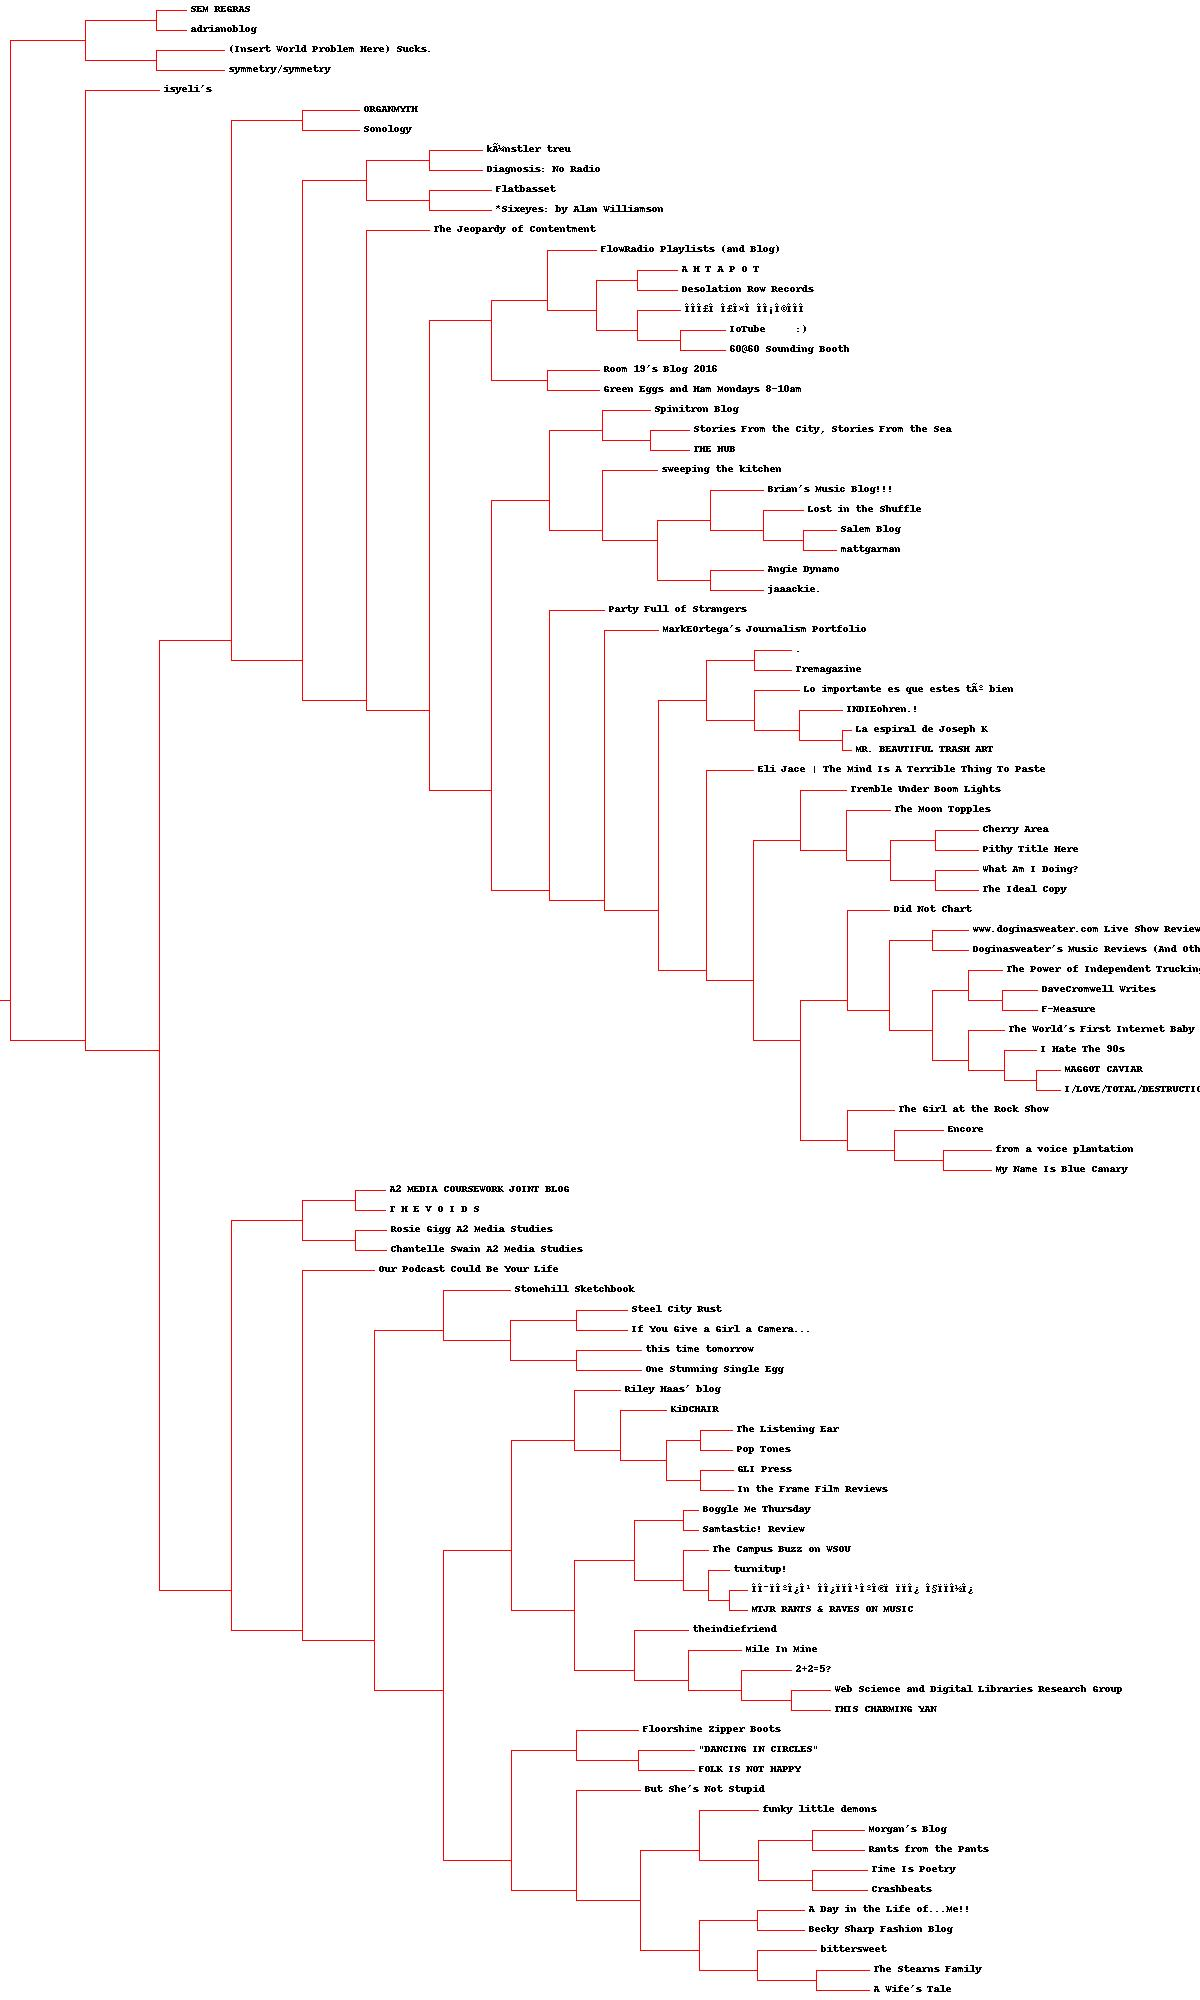
\includegraphics[scale=.3]{images/blogclust.jpg}
\end{enumerate}
\end{homeworkProblem}

%----------------------------------------------------------------------------------------
%	Problem 3
%----------------------------------------------------------------------------------------
\begin{homeworkProblem}% Custom section title
\vspace*{10pt} % Question
Cluster the blogs using K-Means, using k=5,10,20. (see slide 18).  Print the values in each centroid, for each value of k.  How many iterations were required for each value of k?
\subsection{3.1 Approach}
For this problem \textit{PrntK-Cluster.py} was implemented, using 
\\
\lstinputlisting[language=python,
                 style=mybox, 
                 captionpos=t,
                 caption={Using K-Means: PrintK-Clusters.py},
                 label={lst:counting-pages},
				 linerange={13-44},
				 firstnumber=13              
                 ]
{../PrintK-Clusters.py}

\subsection{3.2 Solution}
\import{./}{a08_p3.tex}

\begin{lstlisting}[style=nonumbers, keywords={select, from, where, limit, and}]
Number of iterations for k=5 is 5.
Number of iterations for k=10 is 11.
Number of iterations for k=20 is 6.
\end{lstlisting}
\end{homeworkProblem}

%----------------------------------------------------------------------------------------
%	Problem 4
%----------------------------------------------------------------------------------------
\begin{homeworkProblem}% Custom section title
\vspace*{10pt} % Question
Use MDS to create a JPEG of the blogs similar to slide 29.  How many iterations were required?
\subsection{4.1 Approach}
For this problem \textit{CreateMDS.py} was implemented, using 
\lstinputlisting[language=python,
                 style=mybox, 
                 captionpos=t,
                 caption={Creating MDS with: CreateMDS.py},
                 label={lst:counting-pages},
				 linerange={15-28},
				 firstnumber=15              
                 ]
{../CreateMDS.py}

Above code was extracted from \cite{ci}
\newpage
\subsection{4.2 Solution}
File name: \textit{blogclust.jpg}
\begin{figure}[hr!]
\hspace{-60mm}
\center
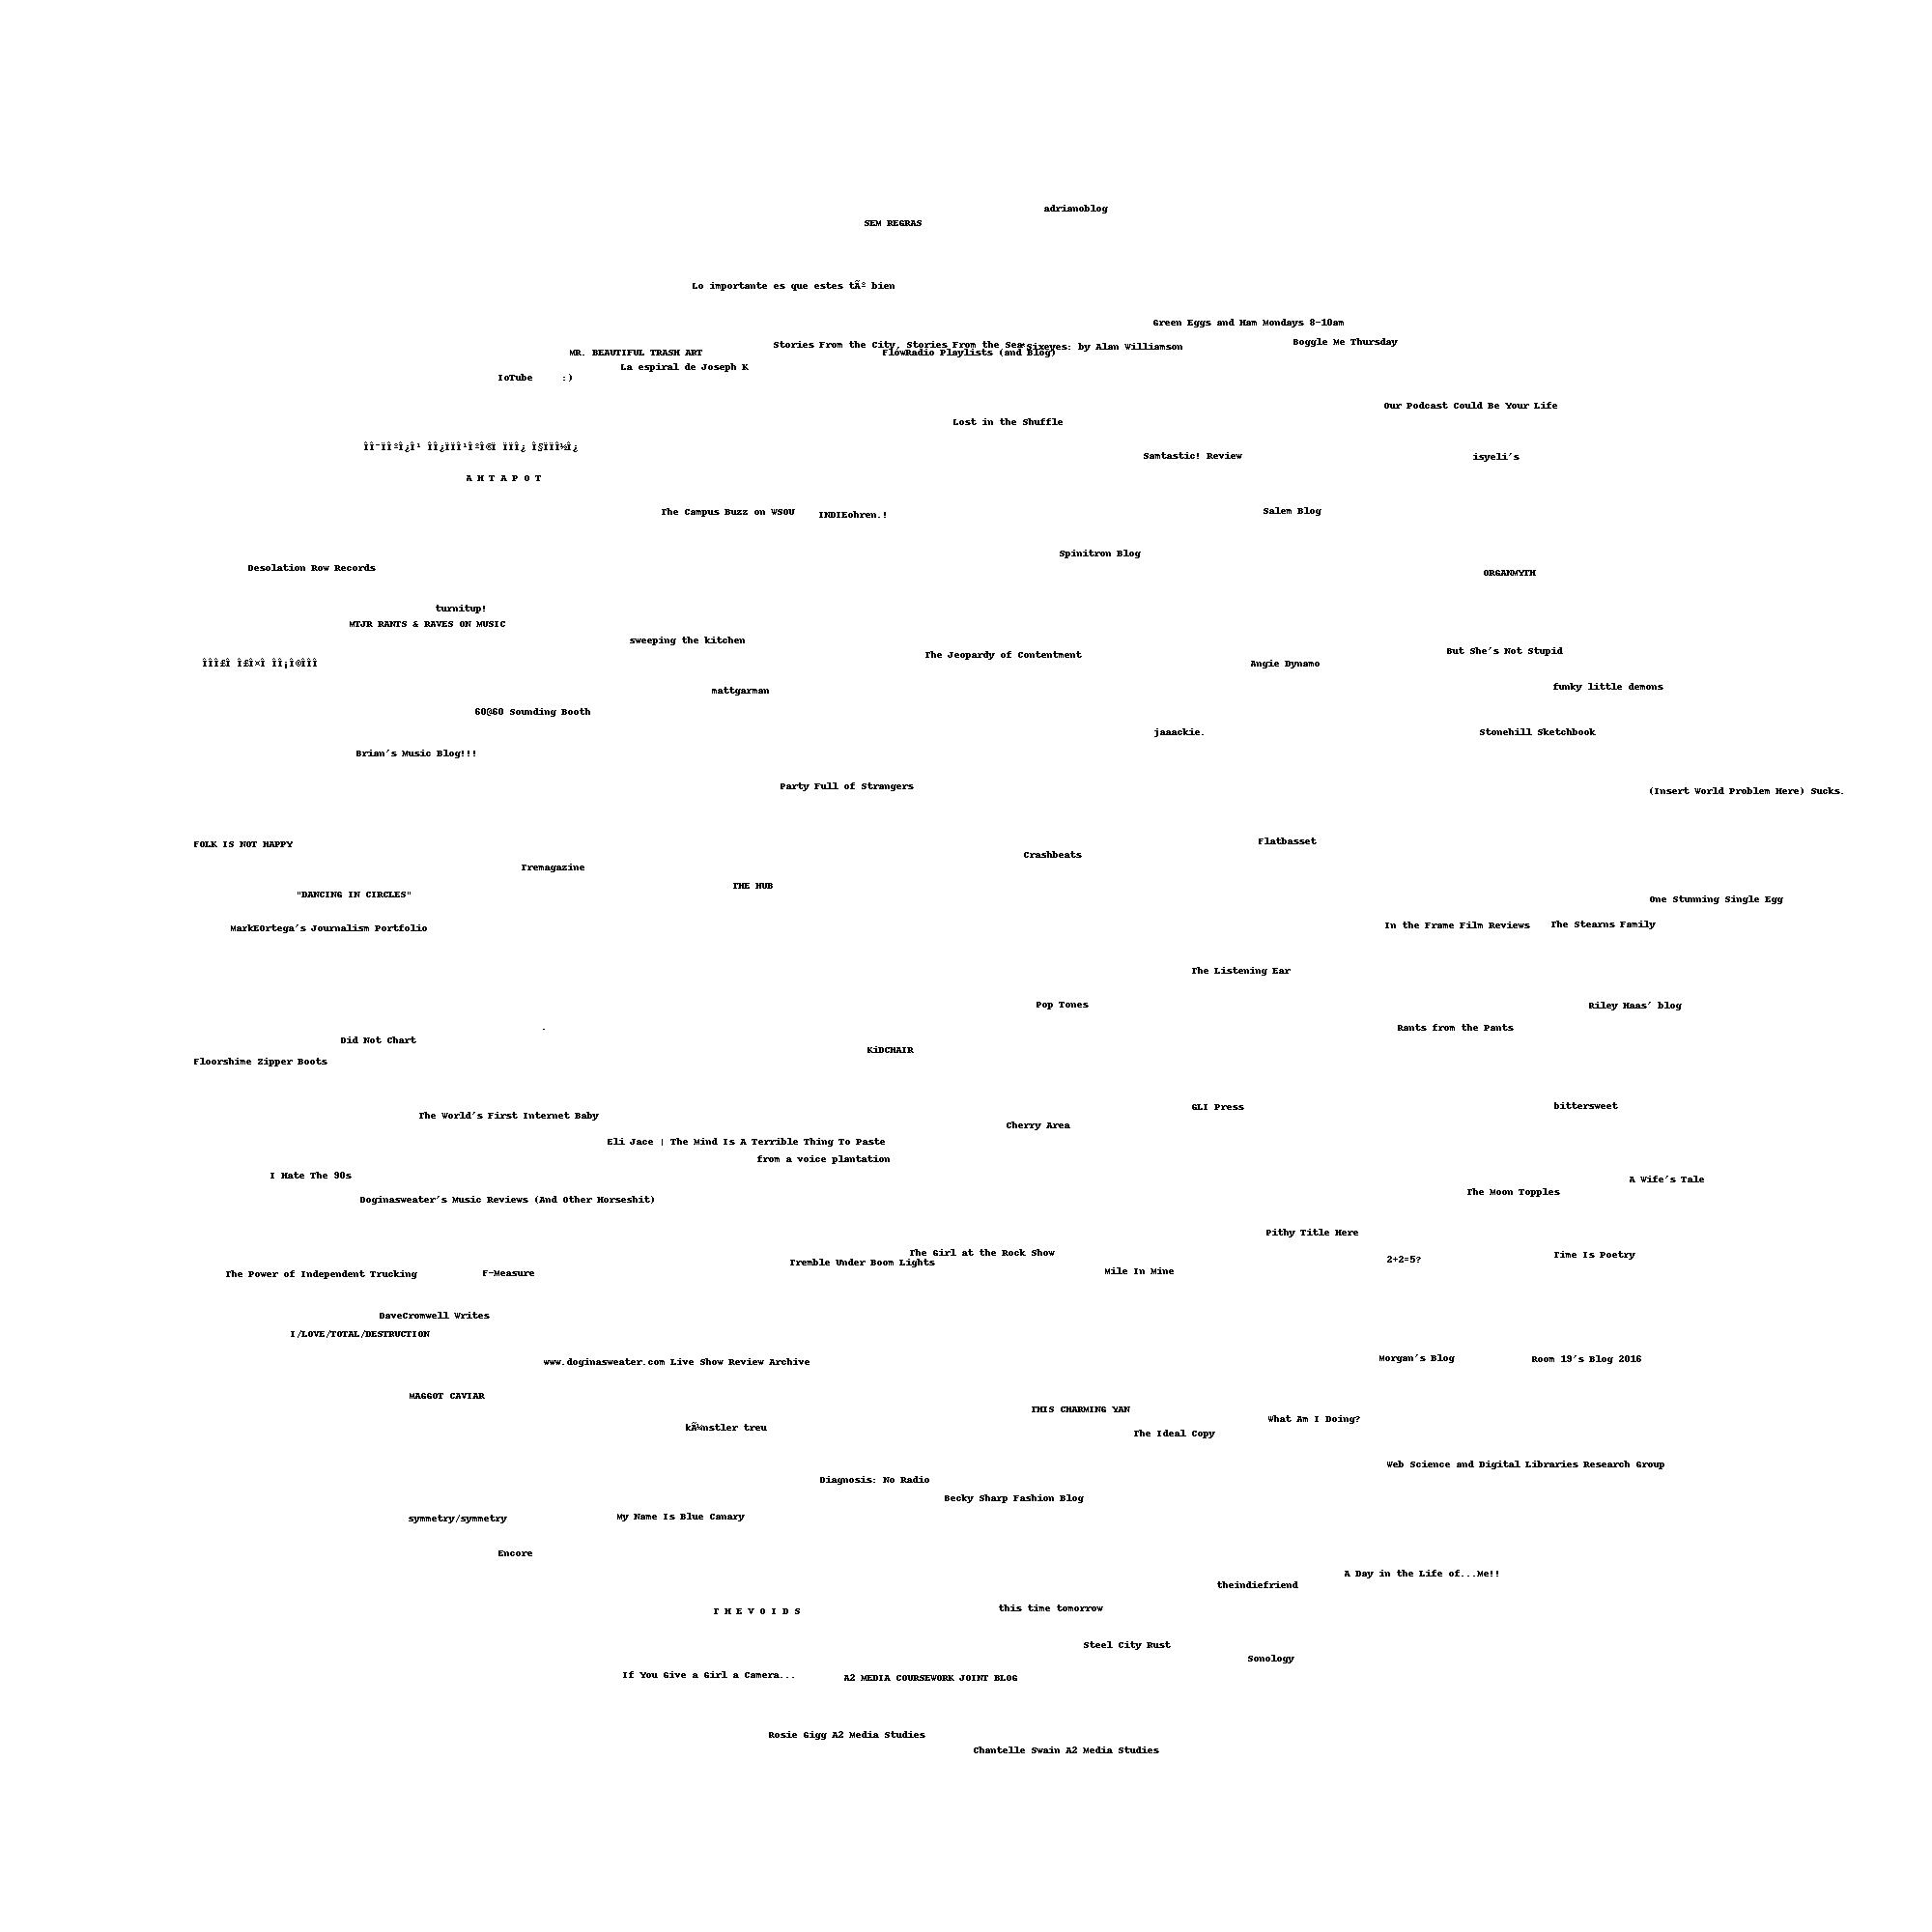
\includegraphics[scale=.25]{images/blogs2d.jpg}
\end{figure}

\begin{lstlisting}[style=nonumbers, keywords={select, from, where, limit, and}]
Number of iterations required was 424
\end{lstlisting}
\end{homeworkProblem}

%----------------------------------------------------------------------------------------
%	Problem 5 - Extra Credit
%----------------------------------------------------------------------------------------
\begin{homeworkProblem}[Problem 5 - Extra Credit]% Custom section title
\vspace*{10pt} % Question
Re-run question 2, but this time with proper TFIDF calculations instead of the hack discussed on slide 7 (p. 32).  Use the same 500 words, but this time replace their frequency count with TFIDF scores as computed in assignment \#3.  Document the code, techniques, methods, etc. used to generate these TFIDF values.  Upload the new
data file to github.\\

Compare and contrast the resulting dendrogram with the dendrogram
from question \#2.\\

Note: ideally you would not reuse the same 500 terms and instead come up with TFIDF scores for all the terms and then choose the top 500 from that list, but I'm trying to limit the amount of work necessary.\\
\subsection{5.1 Approach}
The approach is the same as in problem 2, but we substituted the matrix data calculating with TFIDF values. Our \textbf{Total Document Corpus} is accumulated as we read the matrix in line 38.  \textbf{Document Term} values are accumulated in line 37.
\lstinputlisting[language=python,
                 style=mybox, 
                 captionpos=t,
                 caption={Using TFIDF: CalcTFIDF.py},
                 label={lst:tfidf},
				 linerange={17-54},
				 firstnumber=17              
                 ]
{../CalcTFIDF.py}

Lines 44 through 47 iterates through the matrix to calculate the TFIDF for each blog term. The remaining of the code is a copy of problem 2.
\newpage
\subsection{5.2 Solution}
	
	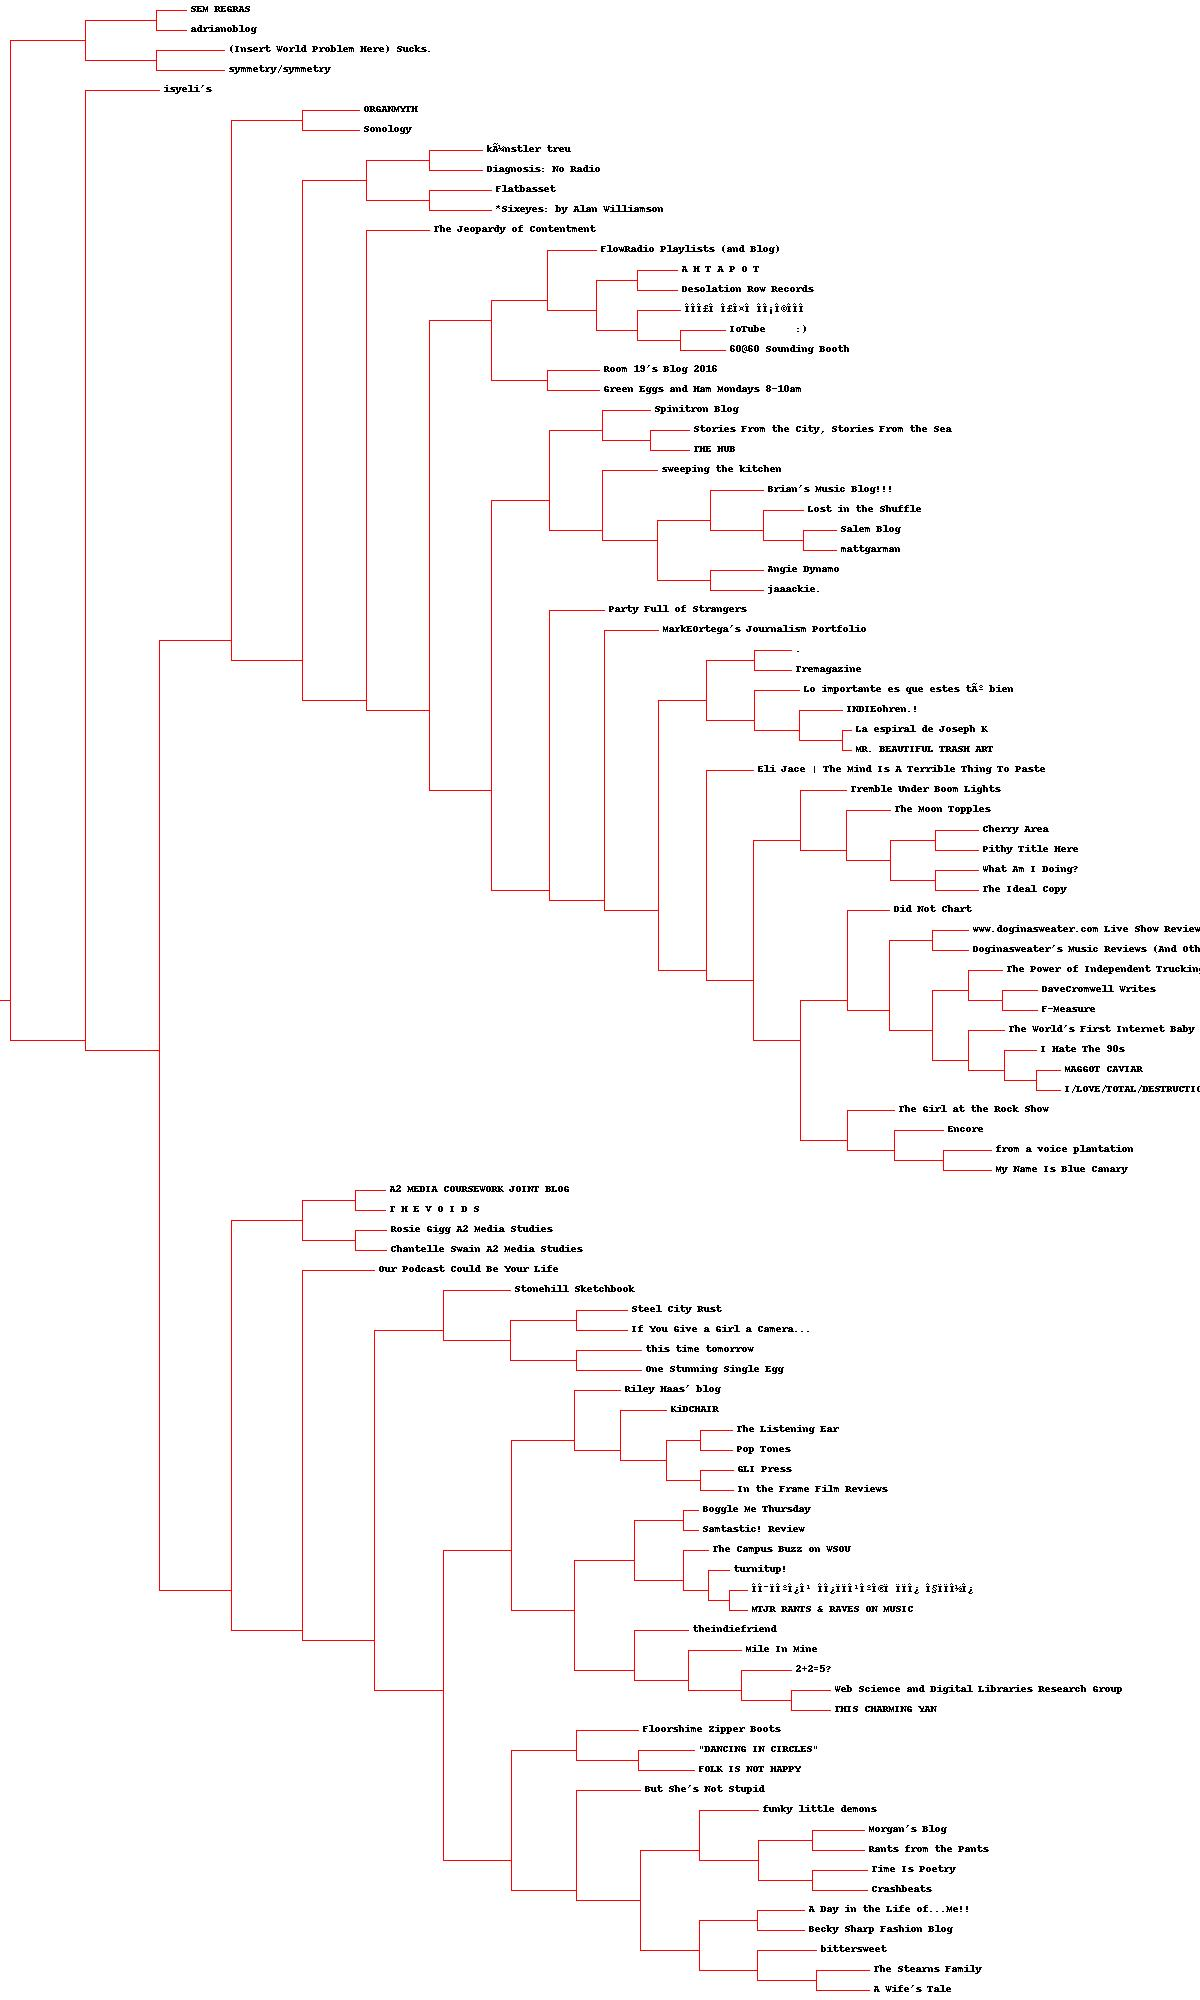
\includegraphics[scale=.3]{images/blogclust.jpg}

The result is very interesting. A great deal of the blogs are clustering with similarity, but they seem to be following on a different categories. For example, blogs F-Measure, DaveCrownell Writes, I hate the 90's, The girl at the Rock Show in problem 2 are clustering together in a flatter way while using TFIDF makes the relationship much hierarchical.
\end{homeworkProblem}

%----------------------------------------------------------------------------------------
%	Bibliography
%----------------------------------------------------------------------------------------
\newpage
\begin{thebibliography}{9}
%\bibitem{Lutz} 
%Lutz, Mark (2013). List and Dictionaries. \textit{Learning Python} (5th ed.). (pp. %262-263). Sebastopol, CA: O'Reilly Media.
%
\bibitem{ci}
Segarn, Toby. Programming Collective Intelligence. \textit{Building Smart Web 2.0 Application}. (pp 29-53). Sebastopol, CA: O'Reilly Media.

%\bibitem{zooming}
%Zooming and dragging. (n.d.) Retrieved March 10, 2016, from \url{http://bl.ocks.org/%mbostock/6123708}

\end{thebibliography}
\end{document}
